\documentclass[11pt]{article}
% ======================================================================
%  The L·F·C gadget pattern of the MCM → MCM-to-APN → APN chain,
%  told categorically and in pictures.  Companion to RequestProject/.
%  Compile with:  tectonic LFCGadgets.tex
% ======================================================================
\usepackage[a4paper,margin=2cm]{geometry}
\usepackage{amsmath,amssymb}
\usepackage{tikz}
\usepackage{tikz-cd}
\usepackage{xcolor}
\usepackage{hyperref}
\hypersetup{colorlinks=true,linkcolor=blue!55!black,urlcolor=teal!60!black}
\usetikzlibrary{arrows.meta,positioning,calc,fit,backgrounds,shapes.geometric,
                shapes.misc,decorations.pathreplacing}

% ---- palette ----------------------------------------------------------
\definecolor{cC}{HTML}{1B6CA8}    % covering  (blue)
\definecolor{cL}{HTML}{2E8B57}    % linearized trace (green)
\definecolor{cF}{HTML}{C98A00}    % Frobenius/Gold (gold)
\definecolor{cK}{HTML}{B5495B}    % Kasami/target (red)
\definecolor{cInk}{HTML}{22303A}
\definecolor{cPaper}{HTML}{F6F4EE}

\tikzset{
  >=Stealth,
  box/.style ={rounded corners=3pt,draw=cInk,fill=cPaper,align=center,inner sep=4pt,font=\small},
  cbox/.style={box,draw=cC,fill=cC!10}, lbox/.style={box,draw=cL,fill=cL!10},
  fbox/.style={box,draw=cF,fill=cF!14}, kbox/.style={box,draw=cK,fill=cK!10},
  ar/.style ={->,thick,cInk},
  lbl/.style={font=\footnotesize\itshape,fill=cPaper,inner sep=1.2pt},
  dot/.style={circle,fill=cInk,inner sep=1.3pt},
}
\tikzcdset{arrow style=tikz,diagrams={>=Stealth}}

\newcommand{\GF}{\mathbb{F}}
\newcommand{\Lk}{L_k}
\newcommand{\dk}{d_k}
\newcommand{\lean}[1]{\text{\footnotesize\ttfamily #1}}
\newcommand{\Fq}{\GF_{2^n}}

\title{\bfseries The $\mathsf{L\cdot F\cdot C}$ gadget pattern\\[-2pt]
\large of \;MCM $\to$ MCM-to-APN $\to$ APN,\; categorically}
\author{\normalsize Companion to \texttt{RequestProject/} — every arrow below is a
\texttt{sorry}-free Lean fact}
\date{}

\begin{document}
\maketitle\thispagestyle{empty}
\vspace{-6mm}
\begin{center}\footnotesize
$L=\Fq$,\quad $q=2^k$,\quad Kasami exponent $\dk=2^{2k}-2^k+1$,\quad
$\Lk(z)=\sum_{i<k}z^{2^i}$,\quad $\gcd(k,n)=1$.\\[2pt]
\emph{H.\ Dobbertin, ``Kasami Power Functions, Permutation Polynomials and Cyclic
Difference Sets'', 1999 — Corollary 2.}
\end{center}
\hrule\vspace{4pt}

% ======================================================================
\section*{1.\quad Three gadgets, one pipeline}
% ======================================================================
\noindent The Kasami APN proof is a composite of \textbf{three self-maps of $L$}.
\begin{center}
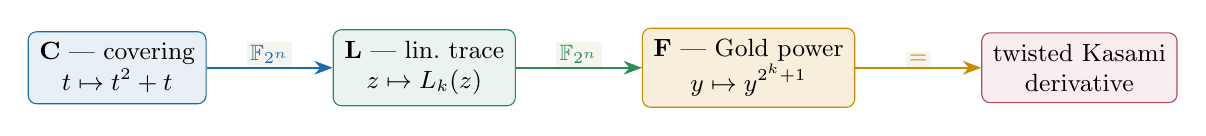
\begin{tikzpicture}[node distance=6mm]
\node[cbox] (c) {\textbf{C} — covering\\ $t\mapsto t^2+t$};
\node[lbox,right=16mm of c] (l) {\textbf{L} — lin.\ trace\\ $z\mapsto \Lk(z)$};
\node[fbox,right=16mm of l] (f) {\textbf{F} — Gold power\\ $y\mapsto y^{2^k+1}$};
\node[kbox,right=16mm of f] (k) {twisted Kasami\\ derivative};
\draw[ar,cC] (c)--(l) node[lbl,midway,above]{$\Fq$};
\draw[ar,cL] (l)--(f) node[lbl,midway,above]{$\Fq$};
\draw[ar,cF] (f)--(k) node[lbl,midway,above]{$=$};
\end{tikzpicture}
\end{center}
\vspace{-1mm}
\begin{center}\footnotesize
\lean{gadgetC},\ \lean{gadgetL},\ \lean{gadgetF} $:F\to F$ \;(morphisms in
\lean{Type}).
\end{center}

% ======================================================================
\section*{2.\quad The chain is one categorical composite}
% ======================================================================
\noindent In the category \lean{Type} ($f\gg g=g\circ f$), the whole pipeline is a
single arrow — this \emph{is} the key identity.
\[
\begin{tikzcd}[column sep=large,row sep=huge]
L \arrow[r,"\textcolor{cC}{\mathsf{C}}\;t^2+t"] \arrow[rrd,"\textcolor{cK}{\mathrm{kasamiTwisted}\,k}"'{yshift=-1pt}]
  & L \arrow[r,"\textcolor{cL}{\mathsf{L}}\;\Lk"] & L \arrow[d,"\textcolor{cF}{\mathsf{F}}\;y^{2^k+1}"]\\
  & & L
\end{tikzcd}
\]
\vspace{-3mm}
\begin{center}\footnotesize
$\mathsf{C}\gg\mathsf{L}\gg\mathsf{F}=\mathrm{kasamiTwisted}\,k$ \;($k\ge1$).\quad
\lean{LFCGadgets.lfc\_chain},\ \lean{lfc\_commSq}.\\[2pt]
Key identity: $\bigl((t{+}1)^{\dk}+t^{\dk}+1\bigr)(t^2{+}t)^{2^k}=(t^{2^k}{+}t)^{2^k+1}$
\;\lean{MCMtoAPN.kasami\_key\_identity}.
\end{center}

% ======================================================================
\section*{3.\quad The composite $=$ two pasted commuting squares}
% ======================================================================
\noindent The pipeline factors as two \lean{CommSq}s glued along the MCM numerator
$\mathrm{mcmNumerator}\,k=\mathsf{F}\circ\Lk$.
\[
\begin{tikzcd}[column sep=6.4em,row sep=large]
L \arrow[r,"t^2+t"] \arrow[d,"\mathrm{id}"'] & L \arrow[r,"\Lk"] \arrow[d,"\mathrm{id}"'] & L \arrow[d,"y^{2^k+1}"]\\
L \arrow[r,"\mathrm{kasamiTwisted}\,k"'] & L \arrow[r,"\mathrm{mcmNumerator}\,k"'] & L
\end{tikzcd}
\]
\vspace{-3mm}
\begin{center}\footnotesize
left square = \lean{MCMKasamiCat.mcmKasami\_commSq}; right square =
\lean{mcmNumerator\_commSq}; paste = \lean{kasamiTwisted\_eq\_gold\_trace\_artinSchreier}.
\end{center}

% ======================================================================
\section*{4.\quad Which stages are $\GF_2$-linear (the reusable structure)}
% ======================================================================
\noindent \textbf{C} and \textbf{L} are additive; only \textbf{F} is not. That is
the whole content of the abstraction: a collapse-count on \textbf{C} rides through
the additive \textbf{L} and the permutation \textbf{F}.
\begin{center}
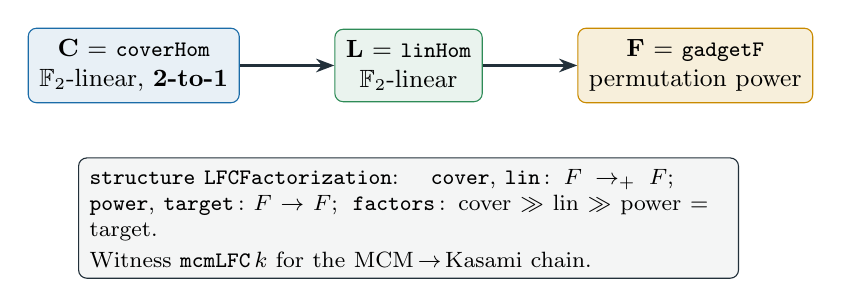
\begin{tikzpicture}[node distance=8mm]
\node[cbox] (c) {\textbf{C} $=$ \lean{coverHom}\\ $\GF_2$-linear, \textbf{2-to-1}};
\node[lbox,right=12mm of c] (l) {\textbf{L} $=$ \lean{linHom}\\ $\GF_2$-linear};
\node[fbox,right=12mm of l] (f) {\textbf{F} $=$ \lean{gadgetF}\\ permutation power};
\draw[ar] (c)--(l); \draw[ar] (l)--(f);
\node[box,below=7mm of l,draw=cInk,fill=cInk!5,align=left,text width=8.1cm]
 {\footnotesize \lean{structure LFCFactorization}: \; \lean{cover},\ \lean{lin}\,$:F\to_{+}F$;\;
  \lean{power},\ \lean{target}\,$:F\to F$;\;
  \lean{factors}\,: $\mathrm{cover}\gg\mathrm{lin}\gg\mathrm{power}=\mathrm{target}$.\\
  Witness \lean{mcmLFC}\,$k$ for the MCM\,$\to$\,Kasami chain.};
\end{tikzpicture}
\end{center}

% ======================================================================
\section*{5.\quad Where the APN count is born: C is exactly 2-to-1}
% ======================================================================
\noindent The only non-injectivity in the pipeline is the covering \textbf{C}:
its fibres are the pairs $\{t,\,t{+}1\}$. \textbf{L} and \textbf{F} are bijections
(for valid $k,n$), so they transport this ``$2$ or $0$'' count verbatim to the
Kasami derivative — i.e.\ APN.
\begin{center}
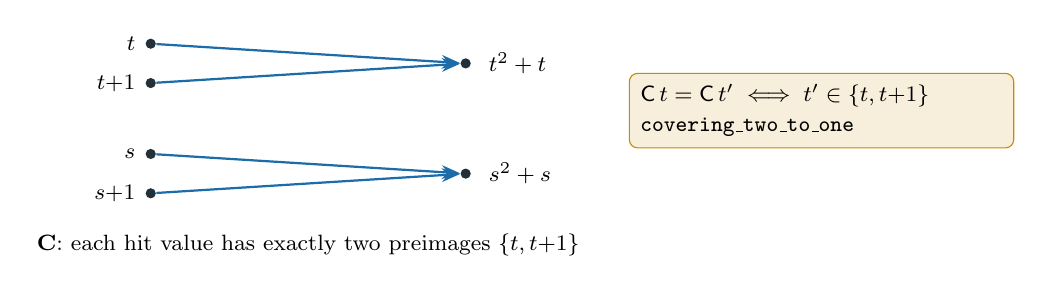
\begin{tikzpicture}
\node[dot,label=left:{\footnotesize $t$}]     (pa) at (0,1.4)  {};
\node[dot,label=left:{\footnotesize $t{+}1$}] (pb) at (0,0.9)  {};
\node[dot,label=left:{\footnotesize $s$}]     (pc) at (0,0.0)  {};
\node[dot,label=left:{\footnotesize $s{+}1$}] (pd) at (0,-0.5) {};
\node[dot] (ta) at (4,1.15) {}; \node[right=1mm of ta,font=\footnotesize]{$t^2+t$};
\node[dot] (tb) at (4,-0.25){}; \node[right=1mm of tb,font=\footnotesize]{$s^2+s$};
\draw[ar,cC] (pa)--(ta); \draw[ar,cC] (pb)--(ta);
\draw[ar,cC] (pc)--(tb); \draw[ar,cC] (pd)--(tb);
\node[font=\footnotesize,align=center] at (2,-1.15)
 {\textbf{C}: each hit value has exactly two preimages $\{t,t{+}1\}$};
\node[fbox,right=20mm of ta,yshift=-6mm,align=left,text width=4.6cm]
 {\footnotesize $\mathsf{C}\,t=\mathsf{C}\,t' \iff t'\in\{t,t{+}1\}$\\
   \lean{covering\_two\_to\_one}};
\end{tikzpicture}
\end{center}

% ======================================================================
\section*{6.\quad The three Lean modules, as a diagram}
% ======================================================================
\noindent The formalisation is exactly this pipeline, split across
\lean{MCM} $\to$ \lean{MCMtoAPN} $\to$ \lean{APN}.
\begin{center}
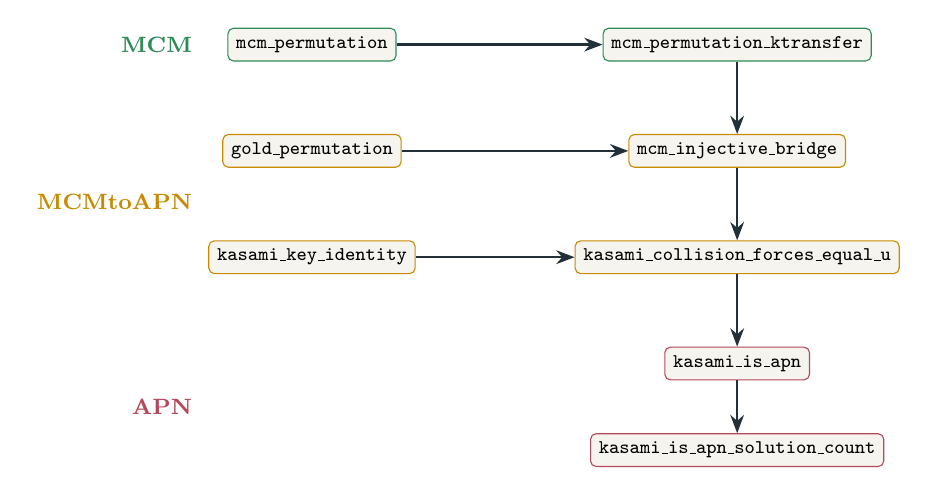
\begin{tikzpicture}[
   nb/.style={draw=cInk,rounded corners=2pt,fill=cPaper,inner sep=3pt,font=\ttfamily\scriptsize}]
\node[nb,draw=cL]                 (mp)  at (0,0)     {mcm\_permutation};
\node[nb,draw=cL]                 (mpk) at (5.4,0)   {mcm\_permutation\_ktransfer};
\node[nb,draw=cF]                 (gp)  at (0,-1.35)  {gold\_permutation};
\node[nb,draw=cF]                 (mib) at (5.4,-1.35){mcm\_injective\_bridge};
\node[nb,draw=cF]                 (kki) at (0,-2.7)  {kasami\_key\_identity};
\node[nb,draw=cF]                 (kcf) at (5.4,-2.7){kasami\_collision\_forces\_equal\_u};
\node[nb,draw=cK]                 (kia) at (5.4,-4.05){kasami\_is\_apn};
\node[nb,draw=cK]                 (ksc) at (5.4,-5.15){kasami\_is\_apn\_solution\_count};
\node[font=\bfseries\footnotesize,text=cL,anchor=east] at (-1.4,0)     {MCM};
\node[font=\bfseries\footnotesize,text=cF,anchor=east] at (-1.4,-2.0)  {MCMtoAPN};
\node[font=\bfseries\footnotesize,text=cK,anchor=east] at (-1.4,-4.6)  {APN};
\draw[ar] (mp)--(mpk);
\draw[ar] (gp)--(mib);
\draw[ar] (mpk)--(mib);
\draw[ar] (kki)--(kcf);
\draw[ar] (mib)--(kcf);
\draw[ar] (kcf)--(kia);
\draw[ar] (kia)--(ksc);
\end{tikzpicture}
\end{center}
\vspace{-2mm}
\begin{center}\footnotesize
\textbf{L}$\cdot$\textbf{F} (MCM $\circ$ Gold, both bijective) $=$ the injective bridge;\;
\textbf{C} (Artin–Schreier, 2-to-1) $=$ the collision collapse; together $\Rightarrow$
\lean{kasami\_is\_apn}.
\end{center}

% ======================================================================
\section*{7.\quad The ambient category theory: invariance groupoid}
% ======================================================================
\noindent Beyond the identity pipeline, the paper's \emph{even-$k$} reduction
``replace $k$ by $n-k$'' is an \textbf{isomorphism in a groupoid}, and differential
uniformity is a \textbf{functor} — constant on isomorphism classes.
\begin{center}
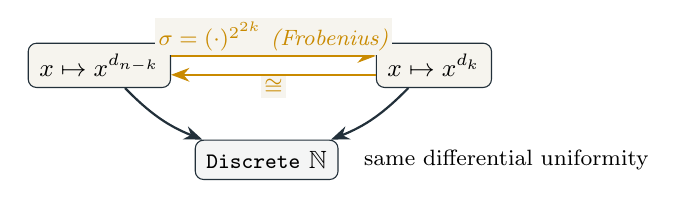
\begin{tikzpicture}[node distance=10mm]
\node[box] (a) {$x\mapsto x^{d_{n-k}}$};
\node[box,right=26mm of a] (b) {$x\mapsto x^{d_k}$};
\draw[ar,cF,transform canvas={yshift=1.2mm}] (a)--(b)
   node[lbl,midway,above]{$\sigma=(\cdot)^{2^{2k}}$ (Frobenius)};
\draw[ar,cF,transform canvas={yshift=-1.2mm}] (b)--(a) node[lbl,midway,below]{$\cong$};
\node[box,fill=cInk!5] (d) at ($(a)!0.5!(b) + (0,-1.2)$) {\lean{Discrete}\ $\mathbb{N}$};
\draw[ar] (a) to[bend right=12] (d);
\draw[ar] (b) to[bend left=12] (d);
\node[right=2mm of d,font=\footnotesize] {same differential uniformity};
\end{tikzpicture}
\end{center}
\vspace{-2mm}
\begin{center}\footnotesize
\lean{FrobeniusGroupoid.kasamiComplementIso},\;
\lean{diffUnifFunctor}\,$:\;\mathrm{SelfMapGroupoid}\,F\Rightarrow\lean{Discrete}\,\mathbb N$,\;
\lean{diffUnif\_kasami\_complement}.
\end{center}

% ======================================================================
\vspace{6mm}
\begin{center}\footnotesize
\renewcommand{\arraystretch}{1.25}
\begin{tabular}{@{}l l l@{}}
\hline
\textbf{gadget / pattern} & \textbf{map} & \textbf{Lean}\\
\hline
\textcolor{cC}{\textbf{C} covering (2-to-1)} & $t^2+t$ & \lean{gadgetC},\ \lean{coverHom},\ \lean{covering\_two\_to\_one}\\
\textcolor{cL}{\textbf{L} linearized trace} & $\Lk(z)$ & \lean{gadgetL},\ \lean{linHom}\\
\textcolor{cF}{\textbf{F} Gold power} & $y^{2^k+1}$ & \lean{gadgetF},\ \lean{gold\_permutation}\\
composite chain & $\mathsf F\!\circ\!\mathsf L\!\circ\!\mathsf C$ & \lean{lfc\_chain},\ \lean{mcmLFC}\\
commuting square & bridge & \lean{mcmKasami\_commSq}\\
APN endpoint & 0 or 2 solutions & \lean{kasami\_is\_apn(\_solution\_count)}\\
invariance groupoid & $k\!\mapsto\!n{-}k$ & \lean{kasamiComplementIso},\ \lean{diffUnifFunctor}\\
\hline
\end{tabular}
\end{center}
\begin{center}\footnotesize
\textbf{One line.} $\;\mathrm{Kasami\ derivative}=\underbrace{y^{2^k+1}}_{\mathsf F}\circ
\underbrace{\Lk}_{\mathsf L}\circ\underbrace{(t^2{+}t)}_{\mathsf C}$: two additive
stages carry the two-to-one collapse of $\mathsf C$ to APN.
\end{center}

\end{document}
